%%%%%%%%%%%%%%%%%%%%%%%%%%%%%%%%%%%%%%%%%
% a0poster Landscape Poster
% LaTeX Template
% Version 1.0 (22/06/13)
%
% The a0poster class was created by:
% Gerlinde Kettl and Matthias Weiser (tex@kettl.de)
% 
% This template has been downloaded from:
% http://www.LaTeXTemplates.com
%
% License:
% CC BY-NC-SA 3.0 (http://creativecommons.org/licenses/by-nc-sa/3.0/)
%
%%%%%%%%%%%%%%%%%%%%%%%%%%%%%%%%%%%%%%%%%

%----------------------------------------------------------------------------------------
%	PACKAGES AND OTHER DOCUMENT CONFIGURATIONS
%----------------------------------------------------------------------------------------

\documentclass[a0,landscape]{a0poster}

\usepackage{multicol} % This is so we can have multiple columns of text side-by-side
\columnsep=100pt % This is the amount of white space between the columns in the poster
\columnseprule=7pt % This is the thickness of the black line between the columns in the poster

\usepackage[svgnames]{xcolor} % Specify colors by their 'svgnames', for a full list of all colors available see here: http://www.latextemplates.com/svgnames-colors

\usepackage{times} % Use the times font
%\usepackage{palatino} % Uncomment to use the Palatino font

\usepackage{graphicx} % Required for including images
\graphicspath{{figures/}} % Location of the graphics files
\usepackage{booktabs} % Top and bottom rules for table
\usepackage[font=large,labelfont=bf]{caption} % Required for specifying captions to tables and figures
\usepackage{amsfonts, amsmath, amsthm, amssymb} % For math fonts, symbols and environments
\usepackage{wrapfig} % Allows wrapping text around tables and figures
\usepackage{comment}
\usepackage{bm}
\usepackage{anyfontsize}
\usepackage{multirow}

\usepackage{sidecap}

\newcommand{\bmu}{\boldsymbol{\mu}}
\newcommand{\bK}{\boldsymbol{\mathrm{K}}}
\newcommand{\bM}{\boldsymbol{\mathrm{M}}}
\newcommand{\mbf}[1]{{\boldsymbol{\mathbf{#1}}}}
\renewcommand{\bm}{\mbf}

\usepackage{subfigure}

\usepackage{parskip}

\usepackage{url}

\usepackage{float} 


\begin{document}

%----------------------------------------------------------------------------------------
%	POSTER HEADER 
%----------------------------------------------------------------------------------------

% The header is divided into three boxes:
% The first is 55% wide and houses the title, subtitle, names and university/organization
% The second is 25% wide and houses contact information
% The third is 19% wide and houses a logo for your university/organization or a photo of you
% The widths of these boxes can be easily edited to accommodate your content as you see fit

\begin{centering}{\fontsize{100}{120} \selectfont \color{NavyBlue} \textbf{Metropolis-Hastings GAN} \color{Black}}\\ % Title

\includegraphics[width=10cm]{uber_ai_logo_bootleg.pdf} \\ % TODO try and move this to the right?
\Huge \textbf{Ryan Turner, Jane Hung, Yunus Saatci, Jason Yosinski}\\ % Author(s)
% \huge Uber AI Labs \\ % University/organization
\end{centering}
%

%

\begin{comment}
\begin{minipage}[b]{0.04959\linewidth}
  
\includegraphics[width=20cm]{uber_ai_logo_bootleg.pdf} % Logo or a photo of you, adjust its dimensions here
\end{minipage}
\end{comment}

\vspace{1cm} % A bit of extra whitespace between the header and poster content

%----------------------------------------------------------------------------------------

\begin{multicols}{3} % This is how many columns your poster will be broken into, a poster with many figures may benefit from less columns whereas a text-heavy poster benefits from more

%----------------------------------------------------------------------------------------
%	ABSTRACT
%----------------------------------------------------------------------------------------

%\color{Navy} % Navy color for the abstract


%----------------------------------------------------------------------------------------
%	INTRODUCTION
%----------------------------------------------------------------------------------------

\Large

\section*{\fontsize{67.1}{82} \selectfont \color{NavyBlue} Generative Adversarial Networks \color{Black}}
\setlength\labelsep   {\dimexpr\labelsep + 0.5em\relax}  
\setlength\leftmargini{\dimexpr\leftmargini + 0.5em\relax}
\vspace{-.5in}
\begin{itemize}
\item Have two neural networks, $G$ and $D$, competing against each other. 
\item $G$ attempts to fool $D$ by generating datapoints which are, from $D$'s perspective, indistinguishable from real datapoints.
\item $D$ in turn simply tries to classify samples coming from $G$ as fake and actual datapoints as real.
\item If this adversarial game converges, it can generate amazingly realistic samples.
\end{itemize}
\textbf{Learning Objective:}
\textcolor{MidnightBlue}{
  \begin{align}
    \underset{G}{\text{min }}\underset{D} {\text{max }} V(D,G) = \mathbb{E}_{\bm{x} \sim p_{\text{data}}(\bm{x})} [\log D(\bm{x})]
    + \mathbb{E}_{\bm{z} \sim p(\bm{z})} [\log(1-D(G(\bm{z})))] \nonumber
  \end{align}}
%\begin{figure}[H]
\begin{centering}
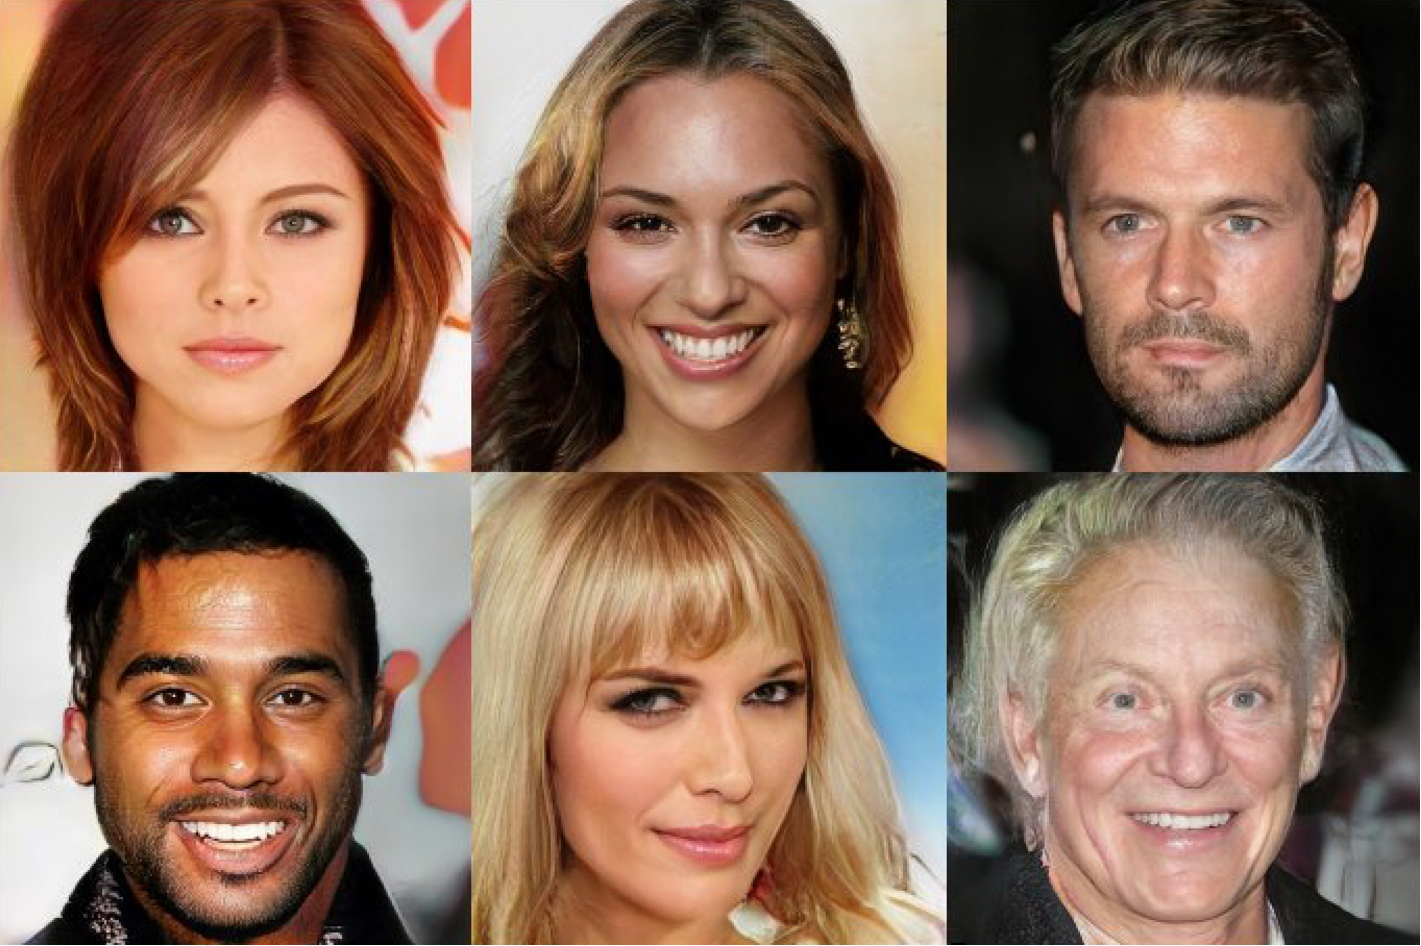
\includegraphics[width=.1\textwidth]{goodsamples.pdf} \\
\small High resolution samples generated by \emph{Karras et. al, arXiv 1710.10196} \\
\end{centering}
%\caption{High resolution samples generated by \emph{Karras et. al, arXiv 1710.10196}}
%\end{figure}
\vspace{-.8in}

$p_D$ could be closer to the real distribution, but we need a way to sample from it. We can draw samples from this distribution using sampling methods.

\section*{\fontsize{67.1}{82} \selectfont \color{NavyBlue} Sampling \color{Black}}
Two sampling methods are rejection sampling and Markov Chain Monte Carlo (MCMC). They can both be used as a post-processing step to improve the generator output. DRS uses rejection sampling, while our MH-GAN uses the Metropolis-Hastings MCMC approach.

Rejection sampling decides whether to accept or reject a sample from the generator. A sample is accepted with probability $p_D/(Mp_G)$, where M is the upper bound for the ratio $p_D/p_G$ over all possible samples. 

The main problem of rejection sampling is there's a large number of sample rejections before first accept because of the high-dimensionality of the sampling space. Thus, DRS has an additional $\gamma$ heuristic to shift the discriminator scores, making the model sample from a distribution different from the real data even when D is perfect. 

We use MCMC instead, which was invented precisely as a replacement for rejection sampling in higher dimensions. The MCMC class of methods sample from a possibly complicated probability distribution by taking multiple samples from a proposal distribution. The Metropolis-Hastings (MH) algorithm is a particular MCMC method that involves taking K samples from the proposed distribution (i.e., the generator) and choosing one sample from the K by sequentially deciding whether to accept the current sample or keep the previously chosen sample based on an acceptance rule 

\section*{\fontsize{67.1}{82} \selectfont \color{NavyBlue} MH-GANs \color{Black}}
\begin{figure}[H]
\centering
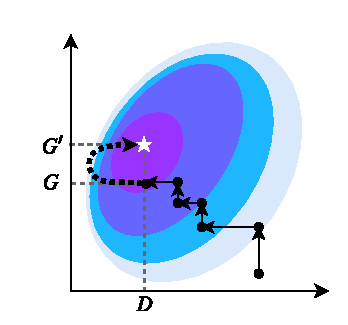
\includegraphics[width=.1\textwidth]{../figures/coord_descent.pdf}
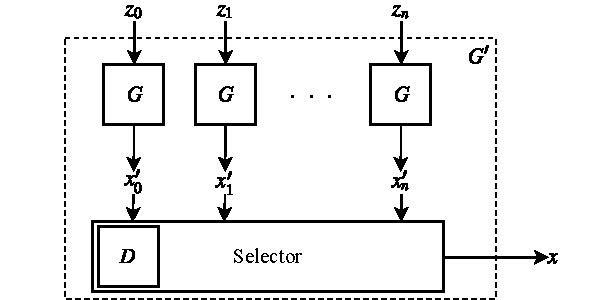
\includegraphics[width=.1\textwidth]{../figures/block_diag.pdf}
\end{figure}
\begin{itemize}
\item Normally in GAN training, the generator moves towards the minimum of the value function (orange) while the discriminator moves towards the maximum (purple). Training stops at a point (D, G) with perfect D and imperfect G. 

\item With an imperfect G plus information from the discriminator, we can obtain a perfect generator G’; then we jump from (D, G) to (D, G’). 

\item G’ works as follows: Noise samples are drawn independently K times and used to generate the chain that the MH selector is applied to. Independent chains are used to obtain multiple samples from G’.

\item  MH selector uses discriminator score D to calculate acceptance probability  
\begin{align} \alpha(\vec x', \vec x_k) = \min\left(1, \frac{D(\vec x_k)^{-1} - 1}{D(\vec x')^{-1} - 1}\right)\,
\end{align}
\end{itemize}


\section*{\fontsize{67.1}{82} \selectfont \color{NavyBlue} Results on Synthetic Data \color{Black}}
\begin{figure}[H]
\centering
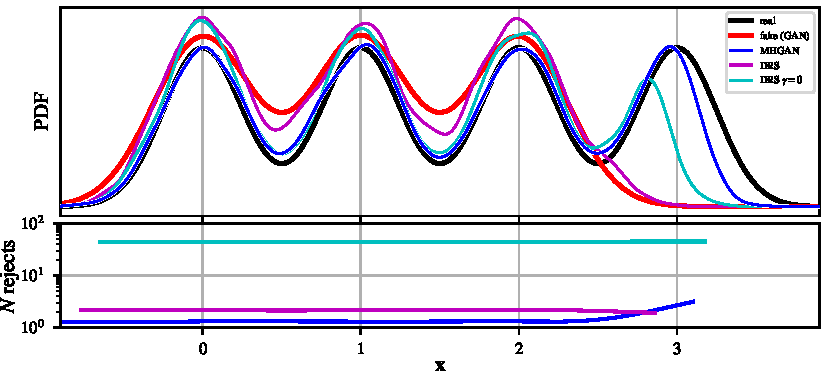
\includegraphics[width=.2\textwidth]{../figures/univariate_example.pdf}
\end{figure}
The real data is a univariate mixture of 4 Gaussians, and the density of the generator $p_G$ shows the common GAN pathology of missing one of the modes. 
DRS without $\gamma$ shift and MH-GAN are able to recover the missing mode, but DRS with $\gamma$ shift (the default used in their paper) cannot. 
However, DRS without $\gamma$ shift increases the number of samples needed before a single accept by an order of magnitude.

\begin{figure}[H]
\centering
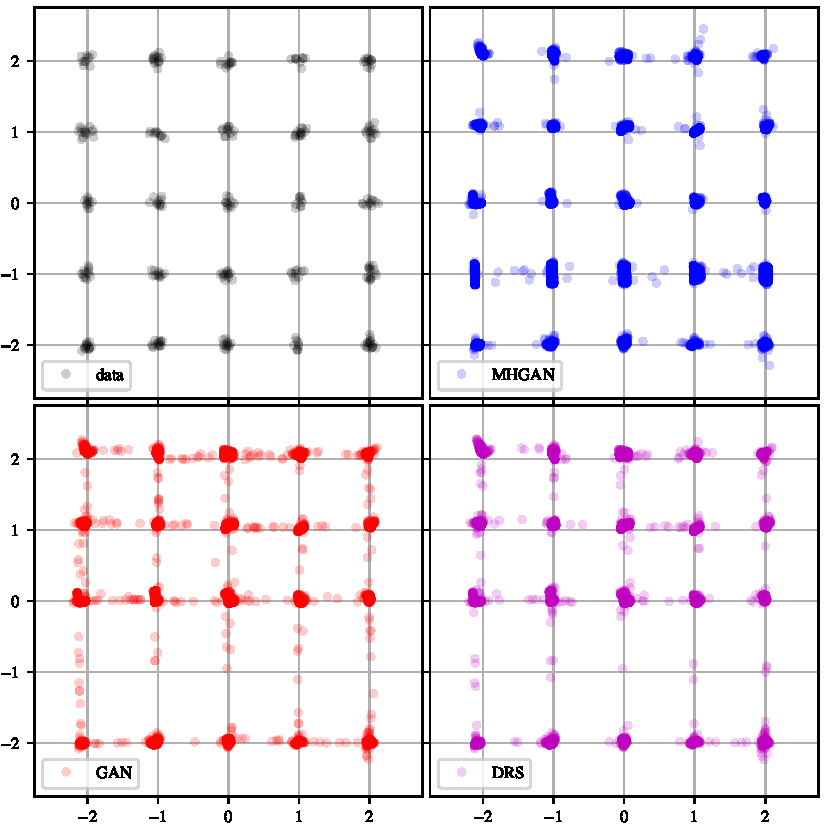
\includegraphics[width=.1\textwidth]{../figures/mog_example_150.pdf}
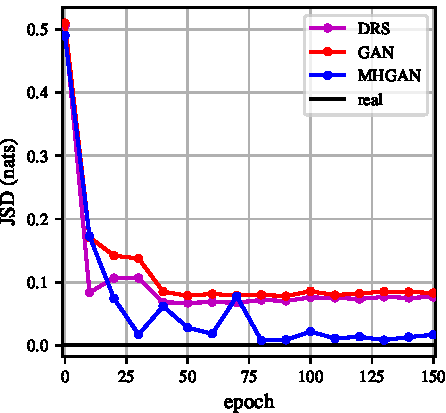
\includegraphics[width=.1\textwidth]{../figures/jsd.pdf}
\end{figure}

\section*{\fontsize{67.1}{82} \selectfont \color{NavyBlue} Results on Benchmark Datasets \color{Black}}
\begin{figure}[H]
\centering
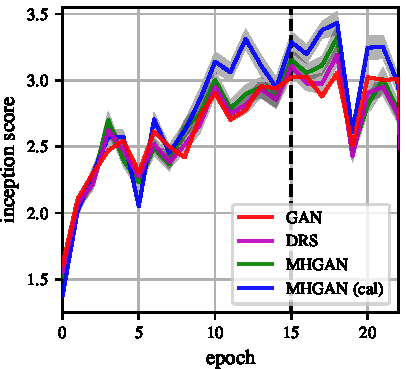
\includegraphics[width=.1\textwidth]{../figures/per_epoch.pdf}
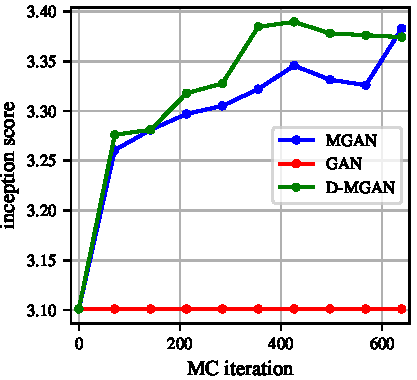
\includegraphics[width=.1\textwidth]{../figures/plot_per_mh.pdf}
\end{figure}



\section*{\fontsize{67.1}{82} \selectfont \color{NavyBlue} Code \color{Black}}
\centering
\large {\url{https://github.com/uber-research/metropolis-hastings-gans}}

\end{multicols}
\end{document}
